\begin{figure}[!b]
	\subfloat[\textbf{CR1. Cluster polar coronal holes.}]
	{
		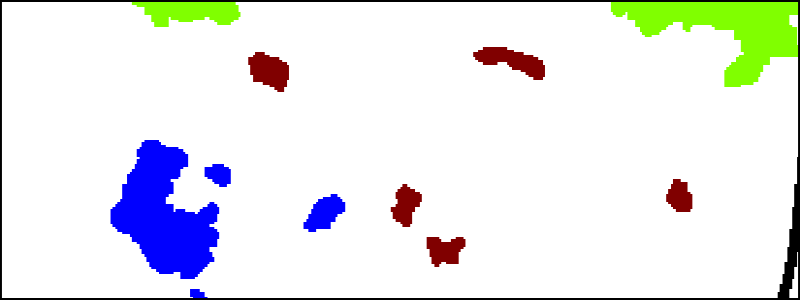
\includegraphics[width=0.45\linewidth]{pictures/thesis/chapter3/clusteringProtocol/20110125_con_northpole_clustering.png}
		\label{subfig:cr1a}
	}
	\subfloat[\textbf{CR1. Cluster polar coronal holes.}]
	{
		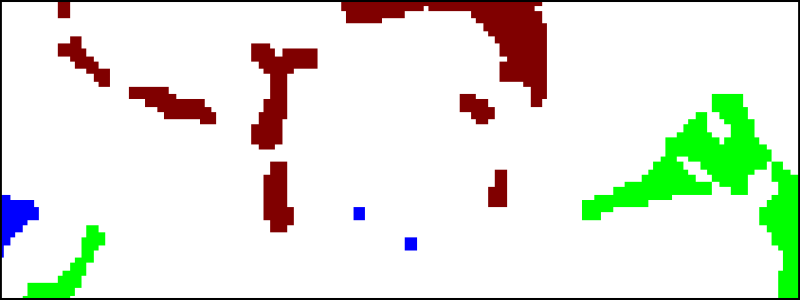
\includegraphics[width=0.45\linewidth]{pictures/thesis/chapter3/clusteringProtocol/20110215_m4_southpole_clustering.png}
		\label{subfig:cr1b}
	}
	
	\subfloat[\textbf{CR2. Nearby clustering}.]
	{
		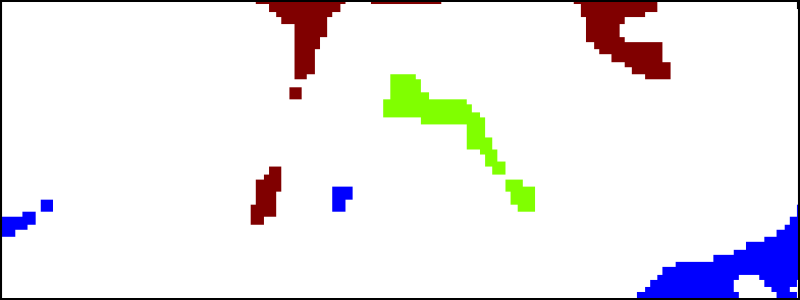
\includegraphics[width=0.45\linewidth]{pictures/thesis/chapter3/clusteringProtocol/20100808_m5_veryclose.png}
		\label{subfig:cr2}
	}
	\subfloat[\textbf{CR3. Small-small clustering.}]
	{
		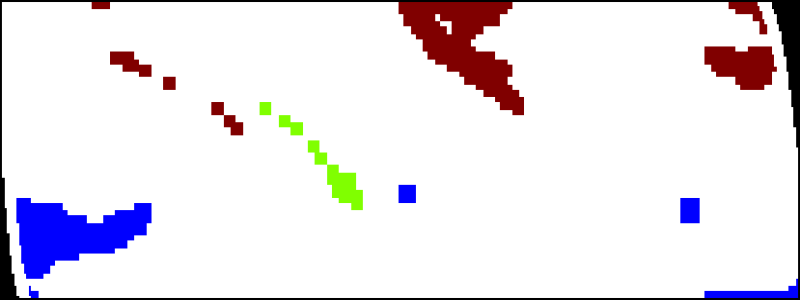
\includegraphics[width=0.45\linewidth]{pictures/thesis/chapter3/clusteringProtocol/20100714_m5_clustersmall.png}
		\label{subfig:cr3}
	}
	
	\subfloat[\textbf{CR4. Large-small clustering.}]
	{
		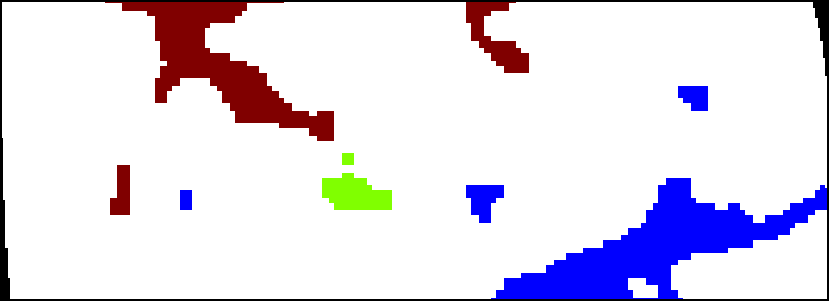
\includegraphics[width=0.45\linewidth]{pictures/thesis/chapter3/clusteringProtocol/20100803_m9_small_big.png}
		\label{subfig:cr4}
	}
	\subfloat[\textbf{CR5. No large-large clustering.}]
	{
		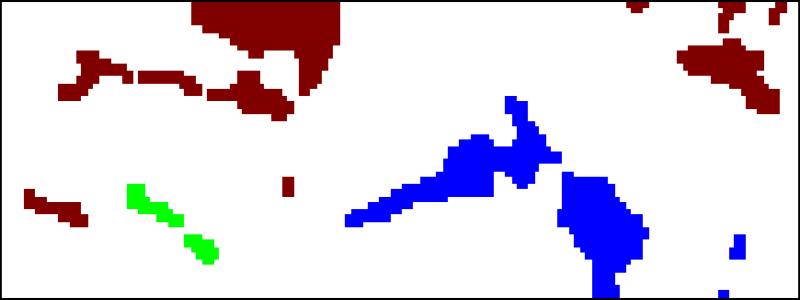
\includegraphics[width=0.45\linewidth]{pictures/thesis/chapter3/clusteringProtocol/20110208_m10_donot_cluster.png}
		\label{subfig:cr5}
	}
	\caption{Manual application of coronal holes clustering rules that
		meet physical requirements. The green coronal holes are combined
		into a single cluster. Here, CR1 to CR5 refer to the rules
		that are summarized in Fig. \ref{fig:holeClusterManual}.
	 We use red to depict coronal holes with positive polarity.
	 We use blue to depict coronal holes with negative polarity.	
	 }
	\label{fig:clusteringInAction}
\end{figure}